\chapter{Die Geschichte und der Untergang des Geldes}
\label{les:12}

\begin{chapquote}{Lewis Carroll, \textit{Alice im Wunderland}}
\enquote{[\ldots] nur weil sie sich nicht an die einfachen Regeln erinnern
wollten, die ihre Freunde sie gelehrt hatten: zum Beispiel, daß ein rotglühender
Feuerhaken einen verbrennt, wenn man ihn zu lange in der Hand hält, oder daß es
gewöhnlich blutet, wenn man sich mit einem Messer sehr tief in den Finger
schneidet, und sie hatte niemals vergessen, daß wenn man viel aus einer Flasche
mit der Aufschrift \enquote{Gift} trinkt, es einem fast mit Sicherheit nicht
bekommt, früher oder später.}
\end{chapquote}

Viele Menschen glauben, dass Geld durch Gold gedeckt ist, welches hinter dicken
Mauern in großen Tresoren eingeschlossen ist. Noch vor einigen Jahrzehnten war
dies tatsächlich der Fall. Ich bin mir nicht wirklich im Klaren darüber, was ich
zuvor dachte, aber ich hatte praktisch keine Ahnung von Gold, Papiergeld oder
warum es überhaupt von etwas gedeckt sein sollte.

Um zu lernen was Bitcoin ist, muss man auch lernen, was Fiatgeld ist: Was es
bedeutet, wie es entstanden ist und warum es vielleicht nicht die beste Idee
war. Also was genau ist Fiatgeld? Und wie sind wir dazu gekommen dieses zu
nutzen?

Wenn etwas als \textit{fiat} deklariert wird, bedeutet dies, dass es durch eine
formelle Genehmigung oder ein Versprechen eingeführt wird. Fiatgeld ist einfach
Geld, weil jemand sagt, dass es Geld ist. Da alle Regierungen heute Fiatgeld
verwenden, ist dieser Jemand deine Regierung. Leider steht es dir nicht frei mit
diesem Wertversprechen nicht einverstanden zu sein. Du wirst schnell merken,
dass dieser Vorschlag alles andere als gewaltfrei ist. Falls du dich weigern
solltest dieses Papiergeld für Geschäfte und deine Steuern zu verwenden, werden
die einzigen Personen mit denen du in Zukunft über Wirtschaft diskutieren
kannst deine Zellengenossen sein.

Der Wert von Fiatgeld ergibt sich nicht aus seinen inhärenten Eigenschaften. Wie
gut eine bestimmte Art von Fiatgeld ist, hängt nur mit der politischen und
fiskalischen (In)Stabilität derjenigen zusammen, die es in Umlauf
\enquote{geträumt} haben. Sein Wert wird durch ein Dekret willkürlich
festgelegt.

\begin{figure}
  \centering
  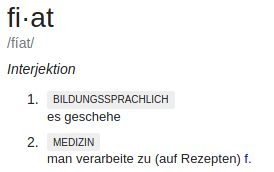
\includegraphics[width=6cm]{assets/images/fiat-definition-de.png}
  \caption{fiat --- Es geschehe}
  \label{fig:fiat-definition}
\end{figure}

\paragraph{}
Bis vor kurzem wurden zwei Arten von Geld verwendet: \textbf{Warengeld}, welches
aus kostbaren \textit{Gütern} hergestellt wurde und \textbf{repräsentatives
Geld}, das, meist in schriftlicher Form, einfach das kostbare Gut
\textit{abbildet}.

\paragraph{}
Wir sind auf das Warengeld bereits in vorherigen Lektionen eingegangen. Die
Menschen benutzten spezielle Knochen, Muscheln und Edelmetalle als Geld. Später
wurden hauptsächlich Münzen aus Edelmetallen wie Gold und Silber als Geld
verwendet. Die älteste bisher gefundene Münze besteht aus einer natürlichen
Gold-/Silbermischung und wurde vor mehr als 2700 Jahren hergestellt.\footnote{
Laut Aufzeichnungen des griechischen Historikers Herodotus aus dem fünften
Jahrhundert vor Christus waren die Lyder das erste Volk welches Gold- und
Silbermünzen verwendet hat. \cite{coinage-origins}} Auch wenn etwas bei Bitcoin
neuartig ist, das Konzept einer Münze ist es nicht.

\begin{figure}
  \centering
  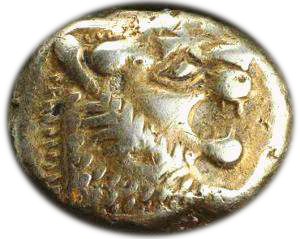
\includegraphics[width=5cm]{assets/images/lydian-coin-stater.png}
  \caption{Eine uralte Münze: Die Lydische Elektron-Trite. Bild: cc-by-sa Classical Numismatic Group, Inc.}
  \label{fig:lydian-coin-stater}
\end{figure}

Es stellte sich heraus, dass das Horten und Halten von Münzen oder “das Hodln”,
um den heutigen Sprachgebrauch zu verwenden, fast so alt ist wie die Münzen
selbst. Der früheste Münz-Hodler war jemand, der fast hundert dieser Münzen in
einen Topf legte und sie in den Fundamenten eines Tempels vergrub. Dieser Topf
wurde erst 2500 Jahre später gefunden. Ziemlich guter \enquote{cold-storage}
wenn du mich fragst.

Einer der Nachteile bei der Verwendung von Edelmetallmünzen ist, dass Teile
davon abgeclipst bzw. abgefeilt werden können, was den Wert der Münze effektiv
verringert. Aus den Abschnitten können neue Münzen geprägt werden, die die
Geldmenge im Laufe der Zeit erhöhen und dabei jede einzelne Münze entwerten. Es
gab Leute, die sich buchstäblich so viel von ihrer Münze abfeilten, wie sie sich
\enquote{erlauben} konnten ohne erwischt zu werden.

Da die Regierungen mit der Inflation nur dann einverstanden sind, wenn sie es
selbst tun, wurden große Anstrengungen unternommen die Guerilla-Entwertung durch
die eigenen Bürger zu stoppen. In klassischer Räuber und Gendarme Manier
wurden die \enquote{Münzfeiler} immer kreativer mit ihren Techniken und zwangen
die \enquote{Meister der Münze} mit ihren Gegenmaßnahmen selbst auch kreativ zu
werden. Isaac Newton, der weltberühmte Physiker und Autor der \textit{Principia
Mathematica} war einer dieser Meister. Ihm wird zugeschrieben, dass er die
kleinen Streifen an der Seite der Münzen die heute noch vorhanden sind
hinzugefügt hat. Vorbei waren die Zeiten des einfachen \enquote{Münzfeilens}.

\begin{figure}
  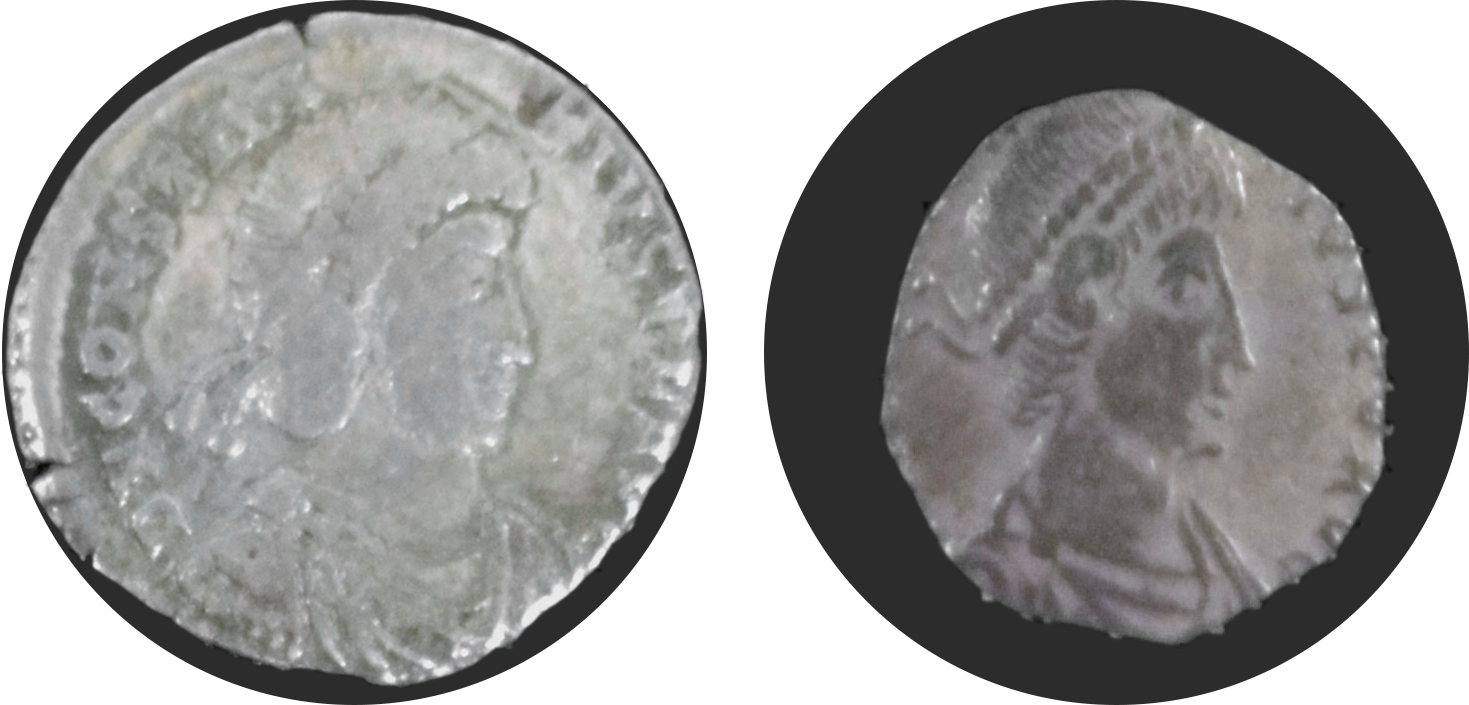
\includegraphics{assets/images/clipped-coins.png}
  \caption{Unterschiedlich stark gefeilte Silbermünzen}
  \label{fig:clipped-coins}
\end{figure}

Auch wenn diese Methoden der Münzentwertung\footnote{ Weitere Methoden um Münzen
unauffällig zu entwerten waren z.B. das Schütteln von Münzen in einem Beutel, um
feinen Gold- bzw. Silberstaub abzuwetzen, und das ausstanzen von Löchern, welche
durch ein Flachhammern der Münze wieder verdeckt wurden.
\cite{wiki:coin-debasement} } unter Kontrolle gebracht werden konnte, leiden die
Münzen noch immer an anderen Problemen. Sie sind sperrig und nicht sehr bequem
zu transportieren, besonders wenn große Werttransfers stattfinden müssen. Mit
einer großen Tasche voller Silberdollar aufzutauchen, wenn man einen Mercedes
kaufen will, ist nicht sehr praktisch.

Wo wir gerade von deutschen Dingen sprechen: Wie der US-Dollar seinen Namen
erhielt ist eine weitere interessante Geschichte. Das Wort \enquote{Dollar}
leitet sich vom deutschen Wort \textit{Taler} ab, kurz für einen
\textit{Joachimsthaler}~\cite{wiki:thaler}. Ein Joachimsthaler war eine Münze,
die in der Stadt \textit{Sankt Joachimsthal} geprägt wurde. Taler ist einfach
eine Abkürzung für jemanden (oder etwas), der aus dem Tal kommt, und da
Joachimsthal \textit{das} Tal für die Herstellung von Silbermünzen war,
bezeichneten die Menschen diese Silbermünzen einfach als \textit{Taler}. Taler (deutsch)
verwandelte sich in Daalders (niederländisch) und schließlich in Dollar
(englisch).

\begin{figure}
  \centering
  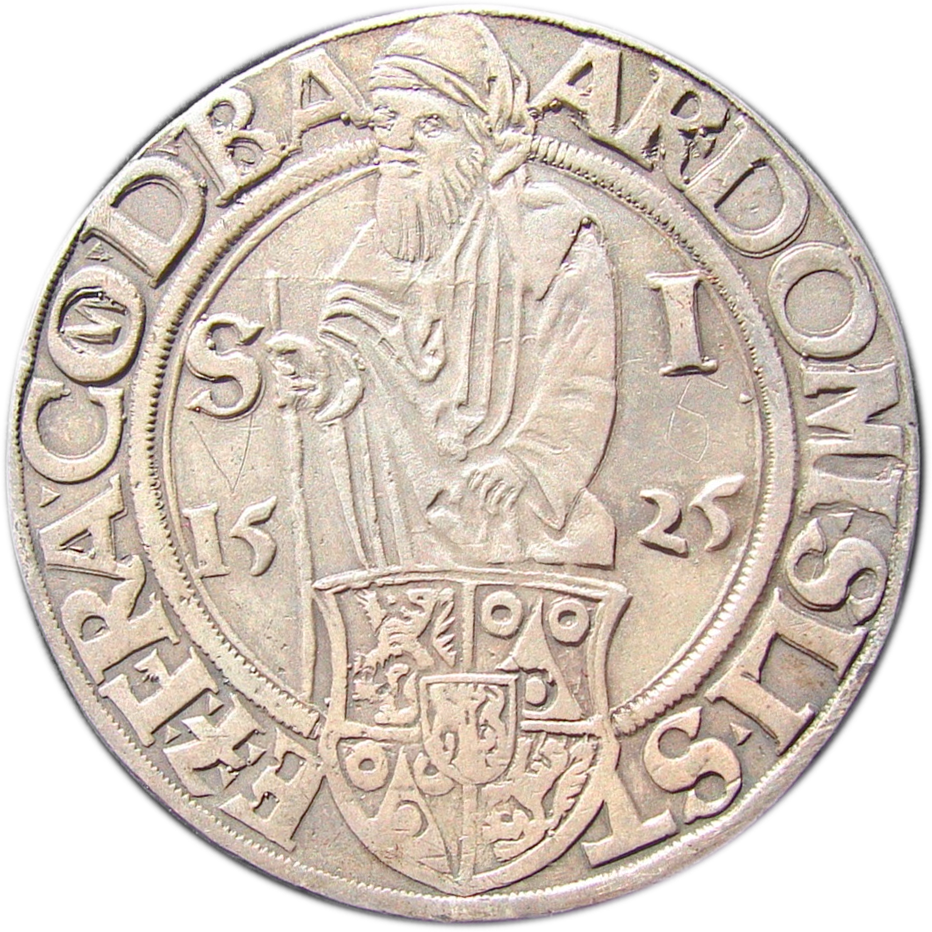
\includegraphics[width=5cm]{assets/images/joachimsthaler.png}
  \caption{Der ursprüngliche \enquote{Dollar}. Bild: cc-by-sa Wikipedia-User Berlin-George.}
  \label{fig:joachimsthaler}
\end{figure}

Die Einführung von repräsentativem Geld läutete den Untergang des Hartgeldes
ein. Gold-Zertifikate wurden 1863 eingeführt und etwa fünfzehn Jahre später
wurde auch der Silberdollar langsam aber sicher durch eine Art Papiervollmacht
ersetzt: Das Silberzertifikat. \cite{wiki:silver-certificate}

Von der Einführung der ersten Silberzertifikate bis zur Umwandlung dieser
Papiere in etwas, das wir heute als einen US-Dollar ansehen würden, vergingen
etwa 50 Jahre.

\begin{figure}
  \centering
  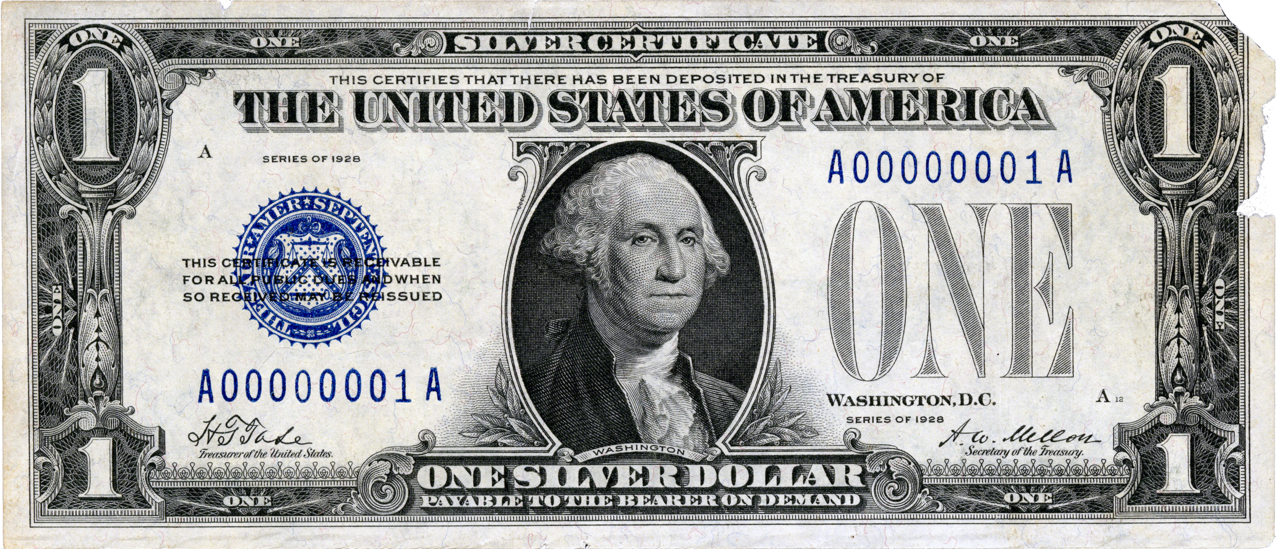
\includegraphics{assets/images/us-silver-dollar-note-smaller.png}
  \caption{Ein Silberdollar von 1928 in den USA. \enquote{Auf Verlangen an den
  Inhaber zahlbar.} Bild: Die Nationale Numismatische Sammlung des Smithsonian
  Institute}
  \label{fig:us-silver-dollar-note-smaller}
\end{figure}

Beachte, dass der US-Dollar in Abbildung~\ref{fig:us-silver-dollar-note-smaller}
von 1928 immer noch den Namen \textit{Silberzertifikat} trägt was darauf
hindeutet, dass es sich hierbei tatsächlich nur um ein Dokument handelt, welches
aussagt, dass dem Träger dieses Papiers ein Silberstück geschuldet wird. Es ist
interessant zu sehen, dass der Text der darauf hinweist mit der Zeit kleiner
geworden ist. Die Spur des \enquote{Zertifikats} verschwand nach einiger Zeit
vollständig und wurde durch die beruhigende Aussage ersetzt, dass es sich um
\enquote{Bundesbanknoten} handelt.

Wie bereits erwähnt geschah das Gleiche mit Gold. Der Großteil der Welt war auf
einem bimetallischen Standard~\cite{wiki:bimetallism} aufgebaut, d.h. Münzen
wurden hauptsächlich aus Gold und Silber hergestellt. Zertifikate für Gold, die
in Goldmünzen eingelöst werden können, waren wohl eine technologische
Verbesserung. Papier ist bequemer, leichter und da es durch einfaches Bedrucken
beliebig unterteilt werden kann, ist es einfacher, es in kleinere Einheiten zu
zerlegen.

Um die Inhaber (Nutzer) daran zu erinnern, dass diese Zertifikate repräsentativ
für das tatsächliche Gold und Silber waren, wurden sie entsprechend gefärbt und
auf dem Zertifikat selbst deutlich gekennzeichnet. Im linken Bereich des Scheins
ist zu lesen:

\begin{quotation}\begin{samepage}
\enquote{Dies bescheinigt, dass in der Staatskasse der Vereinigten Staaten von
Amerika hundert Dollar in Goldmünzen hinterlegt wurden, die auf Verlangen an den
Inhaber zahlbar sind.}
\end{samepage}\end{quotation}

\begin{figure}
  \centering
  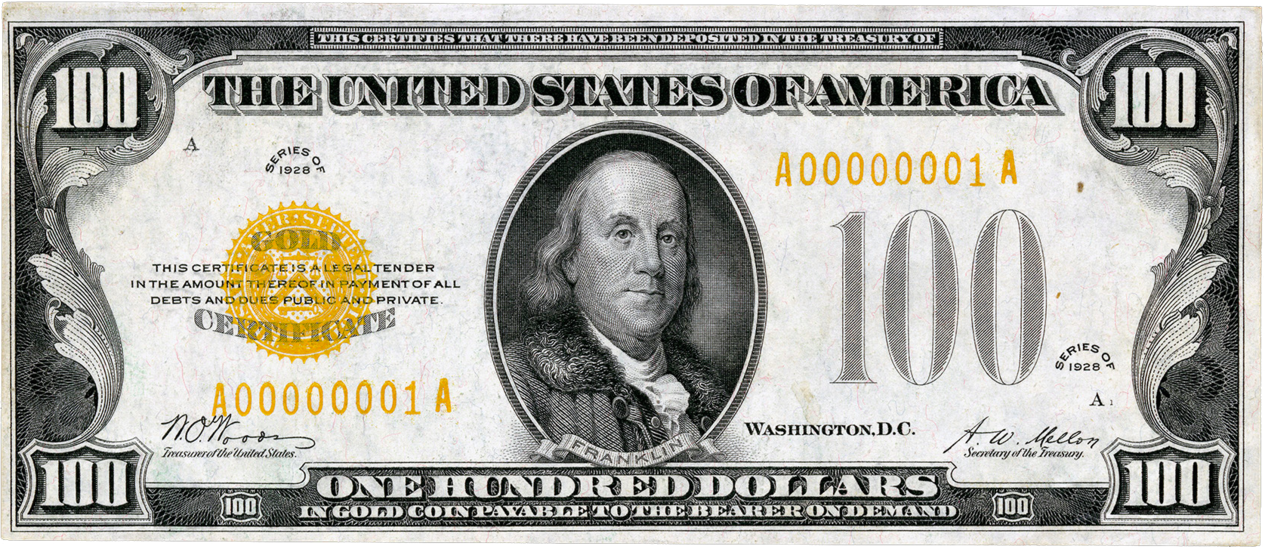
\includegraphics{assets/images/us-gold-cert-100-smaller.png}
  \caption{Ein U.S. Goldzertifikat im Wert von \$100 aus dem Jahre 1928. Bild:
  cc-by-sa Nationale Numismatische Sammlung, Nationalmuseum für amerikanische
  Geschichte.}
  \label{fig:us-gold-cert-100-smaller}
\end{figure}

1963 wurden die Worte \enquote{Zahlbar an den Inhaber auf Anfrage} aus allen neu
ausgegebenen Schuldverschreibungen gestrichen. Fünf Jahre später endete die
Rücknahme von Papiernoten für Gold und Silber.

Die Worte, die auf die Herkunft und die Idee des Papiergeldes hinwiesen, wurden
entfernt. Die goldene Farbe verschwand. Alles was übrig blieb war das Papier und
damit die Fähigkeit der Regierung so viel davon zu drucken wie sie wollte.

Mit der Abschaffung des Goldstandards im Jahr 1971 war dieser hundertjährige
Geniestreich komplett. Geld wurde zu einer Illusion, welcher wir alle bis heute
Glauben schenken: \textbf{das Papiergeld}. Es ist etwas wert, weil jemand, der
eine Armee befehligt und Gefängnisse betreibt sagt, dass es etwas wert ist. Wie
man auf jeder heute im Umlauf befindlichen Dollar-Note deutlich ablesen kann,
\enquote{Diese Note ist ein gesetzliches Zahlungsmittel}. Mit anderen Worten:
Das Geld ist wertvoll, weil die Geldnote, sagt dass sie wertvoll ist.

\begin{figure}
  \centering
  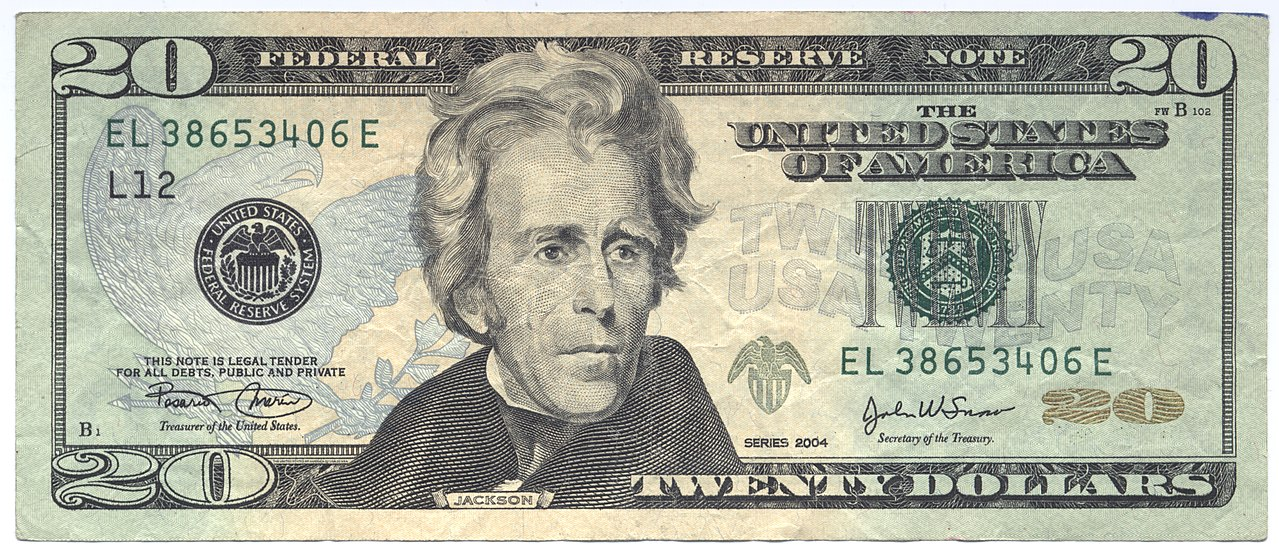
\includegraphics{assets/images/us-dollar-2004.jpg}
  \caption{Eine 2004er Serie von 20-Dollar-Noten in den USA, die heute verwendet
  wird. \enquote{Diese Note ist ein gesetzliches Zahlungsmittel}}
  \label{fig:us-dollar-2004}
\end{figure}

Übrigens, es gibt noch eine weitere interessante Lektion die man heute offen und
für jeden erkennbar auf den Banknoten ablesen kann. Die zweite Zeile beschreibt,
dass dieser Schein ein Zahlungsmittel \enquote{für alle Schulden, öffentlich und
privat} ist. Was für Ökonomen offensichtlich sein könnte, war für mich
überraschend: Alles Geld sind Schulden. Mein Kopf schmerzt deswegen noch immer
und ich werde es dir als eigene kleine Übungsaufgabe überlassen, das Verhältnis
von Geld und Schulden auf der Welt selbst zu erforschen.

\paragraph{}
Wie wir nun sehen konnten wurden Gold und Silber jahrtausendelang als Geld
verwendet. Im Laufe der Zeit wurden Münzen aus Gold und Silber durch Papier
ersetzt. Papiere wurde langsam als Zahlungsmittel akzeptiert. Diese Annahme
schuf eine Illusion --- die Illusion, dass das Papier selbst einen Wert hat. Der
letzte Schritt war die Verbindung zwischen Repräsentation und Realität
vollständig zu durchtrennen: Die Abschaffung des Goldstandards und jeden davon
zu überzeugen, dass das Papier an sich wertvoll ist.

\paragraph{Bitcoin lehrte mich über die Geschichte des Geldes und den größten
Taschenspielertrick in der Geschichte der Wirtschaft: Das Fiatgeld.}

% ---
%
% #### Down the Rabbit Hole
%
% - [Shelling Out: The Origins of Money] by Nick Szabo
% - [Methods of Coin Debasement][coin debasement], [Thaler], [U.S. Silver Certificate][silver certificates], [Bimetallism][bimetallic standard] on Wikipedia
%
% [oldest coin]: https://www.britishmuseum.org/explore/themes/money/the_origins_of_coinage.aspx
% [coin debasement]: https://en.wikipedia.org/wiki/Methods_of_coin_debasement
% [Thaler]: https://en.wikipedia.org/wiki/Thaler
% [Berlin-George]: https://en.wikipedia.org/wiki/File:Bohemia,_Joachimsthaler_1525_Electrotype_Copy._VF._Obverse..jpg
% [silver certificates]: https://en.wikipedia.org/wiki/Silver_certificate_%28United_States%29
% [bimetallic standard]: https://en.wikipedia.org/wiki/Bimetallism
% [Shelling Out: The Origins of Money]: https://nakamotoinstitute.org/shelling-out/
%
% <!-- Wikipedia -->
% [alice]: https://en.wikipedia.org/wiki/Alice%27s_Adventures_in_Wonderland
% [carroll]: https://en.wikipedia.org/wiki/Lewis_Carroll
